\documentclass[10pt,letterpaper,oneside]{article}
\usepackage[margin=0.76in,headheight=15pt,headsep=18pt,footskip=23pt]{geometry}
\usepackage[T1]{fontenc}
\usepackage[utf8]{inputenc}
% pdfLaTeX-only typography (migrated from fontspec): Libertinus Serif via the
% Type 1 "libertinus" package, Noto Sans as the sans family, DejaVu Sans Mono
% for code.
\usepackage[serif]{libertinus}
\usepackage[sf,nott]{noto}
\usepackage{DejaVuSansMono}
\usepackage{microtype,booktabs,array,tabularx,longtable,multicol,enumitem,needspace,ragged2e}
\usepackage[most]{tcolorbox}
\usepackage{tikz}
\usetikzlibrary{positioning,arrows.meta,shapes.geometric}
\usepackage{xcolor,hyperref,fancyhdr,titlesec,lastpage,graphicx,amsmath,amssymb}
\definecolor{ink}{HTML}{163047}
\definecolor{teal}{HTML}{117D83}
\definecolor{teallight}{HTML}{E9F5F4}
\definecolor{gold}{HTML}{C4923A}
\definecolor{papergray}{HTML}{F3F5F7}
\definecolor{graytext}{HTML}{4E626C}
\definecolor{warn}{HTML}{A5532B}
\definecolor{warnbg}{HTML}{FFF4E9}
\hypersetup{colorlinks=true,linkcolor=teal,urlcolor=teal,pdftitle={Residential Cleaning Operations},pdfauthor={Residential Operations Reference}}
\setlength{\parindent}{0pt}
\setlength{\parskip}{5pt}
\setlength{\emergencystretch}{2em}
\setlist[itemize]{leftmargin=1.5em,itemsep=2pt,topsep=3pt}
\setlist[enumerate]{leftmargin=1.6em,itemsep=3pt,topsep=3pt}
\titleformat{\section}{\sffamily\Large\bfseries\color{ink}}{\thesection}{0.75em}{}
\titleformat{\subsection}{\sffamily\large\bfseries\color{teal}}{\thesubsection}{0.7em}{}
\titleformat{\subsubsection}{\sffamily\normalsize\bfseries\color{ink}}{\thesubsubsection}{0.7em}{}
\titlespacing*{\section}{0pt}{16pt}{7pt}
\titlespacing*{\subsection}{0pt}{12pt}{5pt}
\pagestyle{fancy}\fancyhf{}\fancyhead[L]{\sffamily\small\textcolor{ink}{RESIDENTIAL OPERATIONS / FIELD REFERENCE}}\fancyhead[R]{\sffamily\small\textcolor{teal}{2026 EDITION}}
\fancyfoot[L]{\sffamily\scriptsize\textcolor{graytext}{Controlled reference \textbullet\ Confirm product labels and surface care instructions}}
\fancyfoot[R]{\sffamily\scriptsize\textcolor{ink}{\thepage\ / \pageref{LastPage}}}
\renewcommand{\headrulewidth}{0.35pt}\renewcommand{\footrulewidth}{0pt}
\newtcolorbox{notebox}[1][]{enhanced,breakable,colback=teallight,colframe=teal,boxrule=.55pt,arc=1.5mm,left=9pt,right=9pt,top=7pt,bottom=7pt,#1}
\newtcolorbox{safetybox}[1][]{enhanced,breakable,colback=warnbg,colframe=warn,boxrule=.55pt,arc=1.5mm,left=9pt,right=9pt,top=7pt,bottom=7pt,#1}
\newtcolorbox{plainbox}[1][]{enhanced,breakable,colback=papergray,colframe=papergray,boxrule=.25pt,arc=1.5mm,left=9pt,right=9pt,top=7pt,bottom=7pt,#1}
\newcommand{\kicker}[1]{{\sffamily\bfseries\footnotesize\color{teal}\MakeUppercase{#1}}}
\newcommand{\subtle}[1]{{\color{graytext}\small #1}}
\newcommand{\field}[1]{\textbf{#1}\ \rule{0.22\linewidth}{0.3pt}}
\newcommand{\tick}{\ensuremath{\square}\,}
\newcommand{\task}[1]{\par\noindent\tick #1\par}
\newcommand{\sop}[3]{\Needspace{8\baselineskip}\subsection{#1}\subtle{\textbf{Entry condition:} #2}\par\textbf{Work sequence}\begin{enumerate}#3\end{enumerate}}
\newcommand{\accept}[1]{\begin{notebox}\textbf{Acceptance criteria}\quad #1\end{notebox}}
\newcommand{\sources}[1]{\par{\small\color{graytext}\textit{Basis:} #1}\par}
\newcommand{\coverpage}[4]{%
\pagenumbering{Alph}\thispagestyle{empty}\vspace*{1.13in}\kicker{OPERATIONS SYSTEM / PRACTICAL REFERENCE}\par\vspace{.18in}
{\sffamily\fontsize{28}{34}\selectfont\bfseries\color{ink}#1\par}\vspace{.2in}
{\sffamily\Large\color{teal}#2\par}\vspace{.26in}
{\color{gold}\rule{2.2in}{2.2pt}}\par\vspace{.34in}
\begin{notebox}#3\end{notebox}\vfill
{\sffamily\large\color{ink}\textbf{#4}}\par\vspace{5pt}
{\sffamily\small\color{graytext}Version 1.0 \quad|\quad 10 October 2026 \quad|\quad US residential use}\par
\newpage\pagenumbering{roman}\tableofcontents\newpage\pagenumbering{arabic}}
\newcommand{\refurl}[2]{\href{#2}{#1}}
\newcommand{\smalltable}{\par\small\renewcommand{\arraystretch}{1.24}}
\newcommand{\restorenormalfonttable}{\par\normalsize\renewcommand{\arraystretch}{1}}
\begin{document}
\coverpage{Residential Cleaning\\Training Curriculum}{Four-week competency path \textbullet\ skills stations \textbullet\ objective assessments}{A repeatable onboarding and cross-training program built from the manual's PMC rules, tools, kitchen, bathroom, dusting, vacuuming, refrigerator and team-cleaning chapters. Updated surface care, chemical safety, hygiene zoning, and documentation modules are identified as modern supplements.}{Volume 3 of 3 \textbullet\ Trainer and learner handbook}
\section{Program charter and learning outcomes}
\begin{notebox}\textbf{Program format:} 4 weeks, 20 guided hours (5 per week) plus optional supervised field practice. Learners complete observed room demonstrations and a final simulated residence. The 20-hour allocation is a new training design, \emph{not} a requirement from the source manual.\end{notebox}
\textbf{Audience:} home cleaners, new hires, independent operators and lead cleaners. \textbf{Prerequisite:} ability to read product labels and follow safety instructions; provide language access, accommodation and hands-on demonstrations where needed. \textbf{Training standard:} correct and safe completion matters more than a fixed number of minutes.
\subsection{Measurable competencies}
After passing, the learner can:
\begin{enumerate}
\item Distinguish daily reset, weekly/biweekly maintenance cleaning and optional deep-clean services without expanding scope unilaterally.
\item Construct a room-by-room dependency order and explain the manual's one-pass, high-to-low, back-to-front logic.
\item Select, inspect and stage microfiber, brushes, caddy, mop, vacuum, PPE and properly identified products.
\item Protect sensitive materials and electronics; segregate food-contact, general bathroom and toilet tools.
\item Demonstrate kitchen and bathroom standard procedures including distinct bathroom wet/finish passes.
\item Dust and vacuum multi-room layouts, maintaining floor and cord safety and minimizing backtracking.
\item Prepare an approved optional refrigerator-cleaning add-on while protecting food, shelves and controls.
\item Rebalance solo, two-person and three-person work without interference or uncontrolled rushing.
\item Complete a documented inspection, identify defects and perform approved correction / escalation.
\end{enumerate}
\section{Source-to-module mapping}
\smalltable\begin{longtable}{p{.07\linewidth}p{.39\linewidth}p{.18\linewidth}p{.26\linewidth}}\toprule
ID & Module / instructional purpose & Manual anchor & Added contemporary controls\\\midrule\endhead
M1 & Service scope and PMC principles & Intro pp. vii--xi; rules pp. 1--3 & Boundary / consent, handoff / documentation.\\
M2 & Tool apron, portable staging and product functions & Tools pp. 4--9 & Chemical labels / SDS, PPE, color zoning.\\
M3 & Route planning and topological job order & Rules and all room chapters & Prerequisite graph and exception handling.\\
M4 & Kitchen one-pass method & Kitchen pp. 10--24 & Food-contact residues, fragile finishes, appliance controls.\\
M5 & Bathroom two-pass method & Bathroom pp. 25--41 & No default bleach; contact time and toilet hygiene.\\
M6 & High-to-low dusting, bedrooms and living areas & Dusting pp. 42--56 & Dust capture, electronics / privacy.\\
M7 & Vacuuming, hard-floor finishing, stairs & Vacuuming pp. 57--61 & Cords, no wet wood / moisture limits.\\
M8 & Refrigerator and deep-clean boundaries & Refrigerator pp. 62--63 & Safe perishable staging, authorization.\\
M9 & Teams and quality review & Team goals / cleaning pp. 64--67 & QC metrics, recordkeeping and 2-person transitions.\\
M10 & Capstone practical / rework & All above & Formal audit and signoff rubric.\\\bottomrule\end{longtable}\restorenormalfonttable
\sources{All page references refer to the source manual's printed pages, not the PDF viewer's 82-page index. All added safety material is drawn from CDC, OSHA, EPA, Natural Stone Institute, and NWFA links in Section 10.}

\section{Prerequisite skill map}
\begin{center}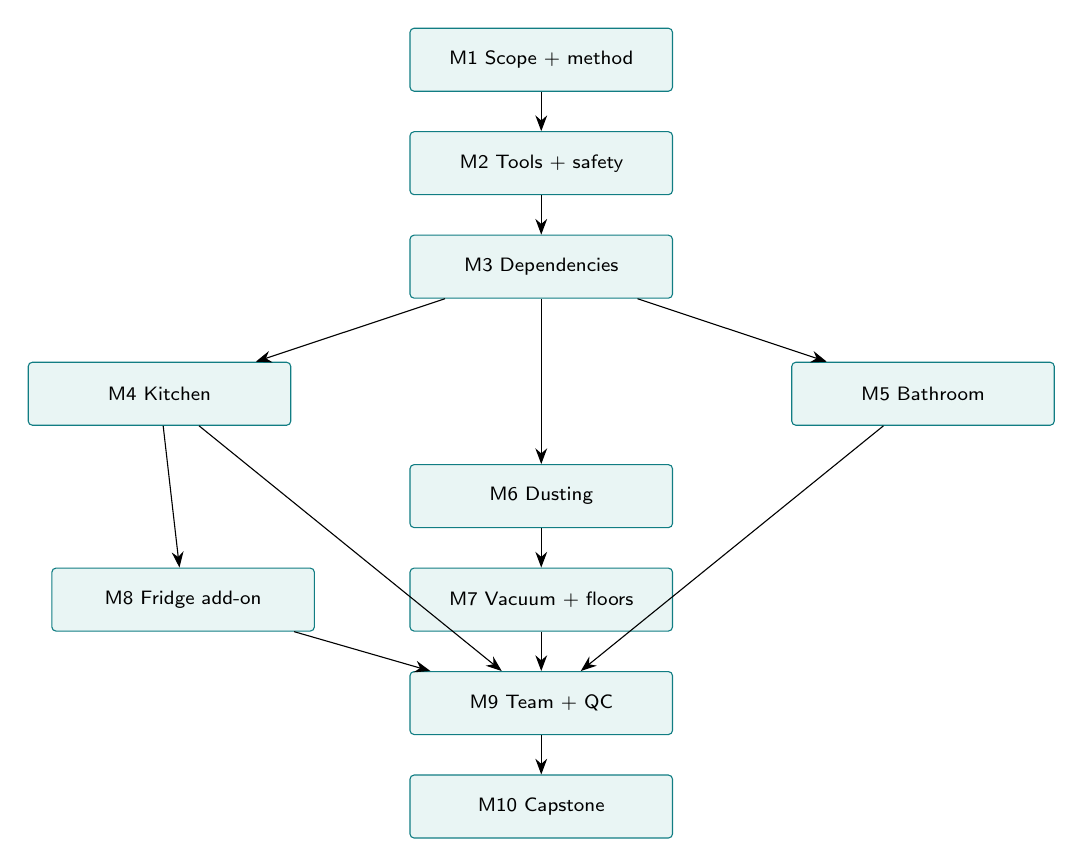
\begin{tikzpicture}[node distance=5mm and 5mm, every node/.style={font=\sffamily\scriptsize}, cell/.style={draw=teal,rounded corners=1.5pt,fill=teallight,align=center,text width=3.1cm,minimum height=8mm}, >={Stealth[length=2mm]}]
\node[cell] (m1) {M1 Scope + method};
\node[cell,below=of m1] (m2) {M2 Tools + safety};
\node[cell,below=of m2] (m3) {M3 Dependencies};
\node[cell,below left=8mm and 15mm of m3] (m4) {M4 Kitchen};
\node[cell,below right=8mm and 15mm of m3] (m5) {M5 Bathroom};
\node[cell,below=21mm of m3] (m6) {M6 Dusting};
\node[cell,below=of m6] (m7) {M7 Vacuum + floors};
\node[cell,left=12mm of m7] (m8) {M8 Fridge add-on};
\node[cell,below=of m7] (m9) {M9 Team + QC};
\node[cell,below=of m9] (m10) {M10 Capstone};
\draw[->] (m1)--(m2);\draw[->](m2)--(m3);\draw[->](m3)--(m4);\draw[->](m3)--(m5);\draw[->](m3)--(m6);\draw[->](m6)--(m7);\draw[->](m4)--(m9);\draw[->](m5)--(m9);\draw[->](m7)--(m9);\draw[->](m4)--(m8);\draw[->](m8)--(m9);\draw[->](m9)--(m10);
\end{tikzpicture}\end{center}
\textbf{Gate rule:} do not advance a learner to chemical application, appliance interiors or unsupervised floor work until the safety and finish-selection stations pass. Optional refrigerator exercise can be skipped for a maintenance-only learner, with restricted qualification noted on the signoff.

\section{Four-week instruction plan}
\smalltable\begin{longtable}{p{.09\linewidth}p{.09\linewidth}p{.26\linewidth}p{.42\linewidth}}\toprule
Week & Hours & Modules & Instructor and learner activities\\\midrule\endhead
1 & 2.0 & M1: scope / rules & Sort 20 task cards into daily, PMC, deep. Walk a mock room clockwise and identify forbidden backtracking.\\
1 & 2.0 & M2: tools / safety & Stage a caddy; read sample labels and SDS, find precautions, sort cloths, identify unsafe chemical pairs and finishes.\\
1 & 1.0 & M3: workflow & Draw a dependency graph; identify why dusting precedes vacuuming and sink work precedes final kitchen mopping.\\\midrule
2 & 2.5 & M4: kitchen & Guided full kitchen route, one-pass station, surface compatibility test, appliance touchpoints and sink endpoint.\\
2 & 2.5 & M5: bathroom & Demonstrate wet pass, tool separation, toilet exterior sequence, dry pass, floor exit and signoff.\\\midrule
3 & 2.0 & M6: dusting & Train eye path to ceiling / ledges, controlled dust pickup and object reset; living / bedroom simulation.\\
3 & 2.0 & M7: vacuum / floors & Floor-head choice, cords / stairs, corners, debris, low-moisture mop covers and wet-floor controls.\\
3 & 1.0 & M8: refrigerator & Optional add-on authorization, staging mock food, shelf sequence and protecting appliance components.\\\midrule
4 & 2.0 & M9: team planning & Role-play solo, two-person and three-person schedules; identify longest indivisible job and divide finishing tasks.\\
4 & 3.0 & M10: capstone & Full simulated home, practical checklist, oral hazard questions, score and corrective coaching.\\\bottomrule\end{longtable}\restorenormalfonttable
\subtle{Hour total = 5 + 5 + 5 + 5 = 20. Training ratios are adjustable to house size, language and learner experience.}

\section{Trainer lesson cards}
\subsection{M1--M3 / Foundation and safe setup}
\textbf{Demonstrate:} classify tasks; trace start-to-finish route; select a cleaner from surface identity rather than surface color; identify mandatory safety-stop conditions. \textbf{Practice:} give a learner a caddy with one misidentified sprayer, mixed toilet cloth and metal scraper intended for stone; have them flag and correct each problem. \textbf{Exit test:} no unlabeled products, unsafe chemical combinations, or unresolved unknown finishes.
\subsection{M4 / Kitchen practice station}
\textbf{Equipment:} staged counters with movable containers, fake grease, fingerprints on cabinet pulls, cold stove facade, sink, demonstration floor. \textbf{Procedure:} cabinet touches \(\rightarrow\) backsplash/counters \(\rightarrow\) appliance exteriors \(\rightarrow\) cooktop \(\rightarrow\) sink \(\rightarrow\) dry floor \(\rightarrow\) appropriate damp floor. \textbf{Trainer prompts:} Which items should not move? What is the last wet counter task? Why are metal blades not the standard option? \textbf{Exit test:} complete with zero unsafe surface treatments and no food-contact chemical residues.
\subsection{M5 / Bathroom practice station}
\textbf{Equipment:} shower wall, dummy fixture, mirror, vanity, toilet, dedicated cloths, disposable simulated contamination. \textbf{Procedure:} wet shower/tub/basin/bowl work; then clean vanity/mirror/faucet; segregated toilet exterior; sweep/vacuum and floor finish last. \textbf{Trainer prompts:} How do you respond when a cleaner's label requires 5 minutes of wet time? What to do after discovering an unknown product residue? \textbf{Exit test:} no red-to-green cloth crossover; dry non-slip surfaces; no unlabelled chemical.
\subsection{M6--M7 / Dry rooms and floors}
\textbf{Equipment:} high ledges, books, imitation fragile decor, electronics dummy, two floor types, safely staged stair. \textbf{Demonstrate:} dust capture high to low; finish each item before moving on; respect private objects and manufacturer screen guidance; choose bare-floor vs carpet attachments; control cords and inspect for surface moisture. \textbf{Exit test:} no dropped debris onto finished areas or pooled mop water.
\subsection{M8--M9 / Optional interior work and staffing}
\textbf{Refrigerator scenario:} client did not authorize clearing shelves; learner must refuse that addition and offer a separate plan. In authorized scenario, stage perishables and wipe top shelf downward before standard kitchen. \textbf{Team exercise:} model three workers in which vacuuming becomes the longest indivisible task. Learner should move start time earlier and assign short finishing tasks to avoid idle staff. \textbf{Exit test:} team does not enter unfinished hazardous zone or create floor slip/cord conflict.

\section{Assessment: knowledge, performance and safety}
\subsection{Scoring and qualification rule}
\begin{notebox}\textbf{Proposed certification rule:} knowledge check \(\ge 80\%\), practical work \(\ge 85\%\), \textbf{zero critical safety errors}, and completion of both kitchen and bathroom stations. Scores are program choices, not thresholds stated by the book or by regulators. A critical safety error overrides numerical score until retraining and re-observation.\end{notebox}
\smalltable\begin{tabularx}{\linewidth}{p{.39\linewidth}p{.12\linewidth}X}\toprule
Practical domain & Points & Observable evidence\\\midrule
Scope and safe start & 15 & Consent, surfaces, access, ventilation and PPE assessed.\\
Kit preparation / chemical control & 15 & Labels correct, cloth zones separate, no mixing, correct dilution.\\
Dependency and tool route & 10 & High to low, orderly pass, avoids unnecessary backtracking.\\
Kitchen first-pass execution & 15 & Finish-safe, counters, appliances, sink, floor and reset.\\
Bathroom first-pass execution & 20 & Wet / finish passes, fixture care, dedicated toilet sequence.\\
Dry rooms / floor safety & 10 & Dust capture, vacuum choice, cords, moisture limit.\\
Quality audit / reporting & 10 & Defects identified, waste / items reset, exceptions recorded.\\
Team coordination & 5 & Progress and long-job handoff communicated.\\\midrule
\textbf{Maximum} & \textbf{100} & \textbf{Pass at 85 plus safety gate.}\\\bottomrule\end{tabularx}\restorenormalfonttable
\subsection{Critical errors: automatic hold}
\begin{itemize}
\item Any bleach mixed with another cleaner or any unauthorized mixing of chemical concentrates.
\item Unlabeled or misidentified spray solution used on a client surface.
\item Toilet cloth or brush used on kitchen or non-toilet surface.
\item Metal blade / abrasive used on unknown or incompatible finish; unapproved wet or steam mop on wood.
\item Electrical item sprayed or wetted unsafely; cord or trip hazard left in an occupied route.
\item Unknown mold, damaged electrical equipment or biohazard ignored rather than isolated and escalated.
\end{itemize}
\textbf{Rubric scale for each station:} 0 = not demonstrated or unsafe; 1 = complete only with substantial coaching; 2 = competent with minor prompting; 3 = independent and consistent. The numerical assessment above grades observable outcomes across stations; use the 0--3 scale for coaching notes.
\section{Knowledge check: twelve scenario questions}
\begin{enumerate}[label=\textbf{Q\arabic*.}]
\item A client requests the entire refrigerator interior during a normal PMC visit. Is it (A) always included, (B) an optional separately agreed task, or (C) never cleaned?
\item Why clean high surfaces before vacuuming? (A) time tracking, (B) dust falls / dislodges, (C) vacuum works only with dry chemicals.
\item You cannot identify a stone counter's finish. (A) apply vinegar, (B) test steel wool, (C) stop and verify the compatible procedure.
\item A product says it disinfects only after 4 minutes wet contact. (A) wipe immediately, (B) keep wet for labeled period after precleaning, (C) mix with bleach.
\item Two sprayers contain different products but have similar blue liquids. (A) identify by color, (B) use product labels, (C) smell each.
\item Where are toilet-used microfiber cloths used next? (A) kitchen, (B) mirror, (C) isolated for wash / decontamination.
\item After dusting the living room, what must precede its damp floor pass? (A) dry soil removal, (B) air freshener, (C) polish.
\item If an already clean cabinet face has one fingerprint, what PMC principle applies? (A) wash entire cabinet, (B) proportionate spot cleaning, (C) skip all work.
\item Can a universal very-wet mop technique be used on sealed hardwood? (A) yes, (B) only if it looks clean, (C) no; use manufacturer-approved low moisture.
\item In a two-person job, the kitchen worker finishes late while the other is free. (A) stop working, (B) reassign compatible downstream tasks, (C) crowd wet kitchen floor.
\item What is the correct routine position on whole-house disinfection? (A) mandatory daily, (B) use for all dust, (C) clean regularly and disinfect when warranted by risk / guidance.
\item Cleaner splashes near a live outlet. (A) continue spraying, (B) isolate/stop and follow safe electrical response, (C) add water to dilute.
\end{enumerate}
\begin{plainbox}\textbf{Trainer key:} 1 B; 2 B; 3 C; 4 B; 5 B; 6 C; 7 A; 8 B; 9 C; 10 B; 11 C; 12 B.\par\textbf{Knowledge scoring:} 12 questions, one point each. At least 10/12 meets the 80\% gate (9/12 = 75\%; 10/12 \(\approx\) 83.3\%). Learner must also answer critical chemical safety questions 3--6 and 12 correctly before independent work.\end{plainbox}

\section{Practice scenarios and corrective action}
\smalltable\begin{longtable}{p{.19\linewidth}p{.42\linewidth}p{.28\linewidth}}\toprule
Scenario & Trigger and expected reasoning & Trainer acceptance\\\midrule\endhead
S1: etched stone & Bath descaler beside marble vanity; learner assesses risk, selects compatible cleaning or defers. & No acid use; finish documented.\\
S2: unclear bleach & Older notes call for a premixed bleach sprayer; learner defers until authorized label/protocol confirmed. & No improvised dilution, no mixing.\\
S3: toilet to sink & Helper brings red cloth to bathroom sink; learner stops task and isolates cloth. & Cross-contamination prevented; restart with clean cloth.\\
S4: overloaded schedule & Team has 3 rooms done, vacuum not started, only one suitable machine. & Longest job started sooner; no rushed shortcut.\\
S5: delicate electronics & Dust on TV and cable box near a socket; learner picks dry compatible method. & No direct sprays, unplugging, damage.\\
S6: deep add-on & Refrigerator interior requested without time or food holding plan. & Re-scope and plan before starting.\\
S7: floor puddling & Trainee saturates laminate floor with cleaner. & Stop, dry safely, check for damage, correct moisture method.\\\bottomrule\end{longtable}\restorenormalfonttable
\section{Qualification, supervision and retraining}
\begin{enumerate}
\item Supervisor signs M1--M3 safety and materials gates before exposing client surfaces to chemicals.
\item First kitchen and bathroom cleans are observed. Record unsafe shortcuts even if visually clean.
\item After capstone, authorize \emph{solo PMC}, \emph{team PMC}, and \emph{interior deep cleaning} separately, based on observed stations.
\item Arrange a supervised audit after approximately 30 days of real work; use a corrective-action plan for repeated rework or chemical handling issues.
\item Retrain immediately when a new product, surface or cleaning method is introduced, after an incident, or after a failed observation.
\end{enumerate}
\newpage\section{Printable trainee records}
\subsection*{FORM T-01 / Practical station observation}
\textbf{Trainee:} \rule{2.2in}{.3pt} \quad \textbf{Instructor:} \rule{2in}{.3pt}\par
\textbf{Date / property model:} \rule{4.6in}{.3pt}
\smalltable\begin{tabularx}{\linewidth}{X p{.12\linewidth}p{.12\linewidth}p{.12\linewidth}}\toprule
Competency observed & 0--3 & Pass? & Notes\\\midrule
Scope and exclusions identified & & & \\
Labels / SDS / gloves / compatibility & & & \\
Cloth / toilet zoning & & & \\
Route and dust-to-vacuum dependency & & & \\
Kitchen station completed & & & \\
Bathroom two passes completed & & & \\
Floor finish, vacuum and cords handled & & & \\
Final audit and room reset & & & \\
\bottomrule\end{tabularx}\restorenormalfonttable
\textbf{Critical safety error:} \(\square\) No \(\square\) Yes (hold qualification)\par\vspace{12pt}
\textbf{Coaching / corrective action:}\par\rule{\linewidth}{.3pt}\par\vspace{14pt}\rule{\linewidth}{.3pt}
\newpage\subsection*{FORM T-02 / Capstone score and qualification}
\textbf{Trainee:} \rule{2.3in}{.3pt} \quad \textbf{Date:} \rule{1.5in}{.3pt}
\smalltable\begin{tabularx}{\linewidth}{X p{.18\linewidth}p{.16\linewidth}}\toprule
Domain & Max & Awarded\\\midrule
Scope / safe start & 15 & \\
Kit / chemistry & 15 & \\
Dependency / flow & 10 & \\
Kitchen & 15 & \\
Bathroom & 20 & \\
Dry rooms / floors & 10 & \\
Audit / reporting & 10 & \\
Team communication & 5 & \\\midrule
\textbf{PRACTICAL TOTAL} & \textbf{100} & \\\bottomrule\end{tabularx}\restorenormalfonttable
\textbf{Knowledge:} \rule{.7in}{.3pt}/12 \qquad \textbf{Critical errors:} \(\square\) none \(\square\) hold\par
\textbf{Qualification:} \(\square\) supervised only \(\square\) solo PMC \(\square\) team PMC \(\square\) refrigerator add-on\par\vspace{12pt}
\textbf{Instructor signature:} \rule{2.1in}{.3pt} \quad \textbf{Trainee:} \rule{1.5in}{.3pt}
\par\vspace{12pt}\textbf{Reassessment plan / date:}\par\rule{\linewidth}{.3pt}
\newpage\subsection*{FORM T-03 / Thirty-day field audit}
\textbf{Employee:} \rule{2.2in}{.3pt} \quad \textbf{Observer:} \rule{2in}{.3pt}\par
\textbf{Date / home model:} \rule{4.2in}{.3pt}
\begin{plainbox}
\task{Confirms scope before starting}
\task{Uses labeled cleaners and suitable PPE}
\task{Maintains all cloth/tool hygiene zones}
\task{Plans route; avoids repeated re-entry}
\task{Kitchen approved without unsafe residue or tool use}
\task{Bathroom toilet work segregated}
\task{Vacuum, hard-floor and stair operation safe}
\task{Finishes with own quality inspection}
\task{Records surface uncertainty and scope exclusions}
\task{Escalates hazards and chemical conflicts appropriately}
\end{plainbox}
\textbf{First-pass audit:} \rule{.6in}{.3pt} rooms passed / \rule{.6in}{.3pt} inspected\par
\textbf{Most important coaching item:}\par\vspace{16pt}\rule{\linewidth}{.3pt}\par\vspace{12pt}\rule{\linewidth}{.3pt}

\section{References and scope of updates}
\begin{enumerate}
\item Jeff Campbell with Debbie Sardone, \emph{Speed Cleaning for the Pros}, 2011, user-supplied manual. Source for PMC rules and core task methods; not source of this four-week schedule or score thresholds.
\item \refurl{CDC household cleaning, 2025}{https://www.cdc.gov/hygiene/about/when-and-how-to-clean-and-disinfect-your-home.html} (cleaning vs disinfecting; contact times).
\item \refurl{OSHA worker chemical safety}{https://www.osha.gov/sites/default/files/publications/OSHA3512.pdf} (labels, SDS, chemical mixing and PPE).
\item \refurl{EPA Safer Choice products}{https://www.epa.gov/saferchoice/products} (selection resource, not a guarantee of finish compatibility).
\item \refurl{Natural Stone Institute cleaning}{https://www.naturalstoneinstitute.org/consumers/care/} (sensitivity to acids and abrasives).
\item \refurl{National Wood Flooring Association maintenance}{https://woodfloors.org/maintenance/} (dry/debris removal and avoiding wet mopping).
\end{enumerate}
\begin{notebox}\textbf{Trainer note.} The historical manual contains methods such as particular bleach-spray techniques, steel wool and scraping examples. Those methods are not automatically adopted here. Teach learners to recognize material and chemical constraints first. Every practical is a \emph{controlled teaching simulation}; do not create chemical hazards to test responses.\end{notebox}
\end{document}
